\documentclass[12pt]{article}
\usepackage{tcolorbox}
\usepackage{amsmath}
\usepackage{float}
\include{preamble}
%All credit goes towards Dr. Adam Kapelner for providing the preamble and homework template.

\newtoggle{professormode}




\title{MATH 241 Spring \the\year~ Homework \#3}

\author{Steven Ou} %STUDENTS: write your name here

\iftoggle{professormode}{
\date{Due via Brightspace 11:59PM Sunday, March 1, \the\year \\ \vspace{0.5cm} \small (this document last updated \today ~at \currenttime)}
}

\renewcommand{\abstractname}{Instructions and Philosophy}

\begin{document}
\maketitle

\iftoggle{professormode}{
\begin{abstract}
The path to success in this class is to do many problems. Unlike other courses, exclusively doing reading(s) will not help. Coming to lecture is akin to watching workout videos; thinking about and solving problems on your own is the actual ``working out.''  Feel free to \qu{work out} with others; \textbf{I want you to work on this in groups.}

The problems below are color coded: \ingreen{green} problems are considered \textit{easy} and marked \qu{[easy]}; \inorange{yellow} problems are considered \textit{intermediate} and marked \qu{[harder]}, \inred{red} problems are considered \textit{difficult} and marked \qu{[difficult]} and \inpurple{purple} problems are extra credit. The \textit{easy} problems are intended to be ``giveaways'' if you went to class. Do as much as you can of the others; I expect you to at least attempt the \textit{difficult} problems. 

Bonus points are given as a bonus if the homework is typed using \LaTeX. Links to installing \LaTeX~and program for compiling \LaTeX~is found on the syllabus. You are encouraged to use \url{https://www.overleaf.com/}. If you are handing in homework this way, read the comments in the code; there is a line to comment out and you should replace my name with yours. The easiest way to use Overleaf is to make an Overleaf account, click the link to the \LaTeX~ template, go to \textit{File} and select \textit{Make a copy}. If you are asked to make drawings, you can take a picture of your handwritten drawing and insert them as figures or leave space using the \qu{$\backslash$vspace} command and draw them in after printing or attach them stapled.



\end{abstract}

\thispagestyle{empty}
\vspace{1cm}
NAME: \line(1,0){380}
\clearpage
}

\problem{These exercises will review The Basic/Generalized Principle of Counting.}

\begin{enumerate}

\easysubproblem{In order to use The Basic Principle of Counting, what assumptions must be satisfied?} 

In order to use the basic princpiple of counting, the independent of choices like the number of options available for the second step must remain constant, regardless of which specific option that was chosen i the first step. 
\intermediatesubproblem{Prove the Basic Principle of Counting. Hint: generalize the argument we did in class with the outfits example.}

Argument: Suppose we have 2 step experiment. The first step have outcome $S_1,S_2,\dots,S_m$. For each one of these m outcomes, we branch out into the second step, which has outcomes $P_1,P_2,\dots,P_n$. Using a table we can list the outcomes in a grid where the rows represent the m choices for the first step and the columns represent the n choices for the second steps. Then counting the cells, each cell in the table represent a unique outcome, such as ($S_1,P_1$). Since there are m rows and n columns, the total number of distinct outcomes in the sample space is m x n. 
\easysubproblem{In using the Basic Principle of Counting, one of the assumptions is that the steps must be distinct. What does it mean that the steps are distinct? What can we do to check if the steps are distinct?}

Steps are distinct if every complete "branch" of the experiment's tree diagram results in a unique outcome. To check for distinctness by verifying that "no two branches are identical". If choosing different paths leads to the exact same result, the steps are not distinct. 

\intermediatesubproblem{Suppose a license plate comprises of 4 entries where the first two entries  are letters and the last two entries are digits. For simplicity, suppose the only letters allowed are $A$ and $B$ and the only digits allowed are 0 and 1. Draw a tree diagram which shows all the possible license plates that we can have. }
\\
\begin{figure}[H]
    \centering
    \includegraphics[scale=0.2]{uname.jpg}
\caption{}
\end{figure}


\easysubproblem{How many possible license plates do we have in the above experiment? In your answer, be sure to explain why the steps are distinct.}

We can have a possible of 16 license plates in above experiment because of the unique positions, independence of outcomes, and we check for distinctness by ensuring that no two branches are identicals in the final outcome even in the tree. 

\intermediatesubproblem{Suppose a license plate comprises of 4 entries where the first two entries  are letters and the last two entries are digits. For simplicity, suppose the only letters allowed are $A$ and $B$ and the only digits allowed are 0 and 1. Further suppose that no repetition is allowed. Draw a tree diagram which shows all the possible license plates that we can have. }
\begin{figure}[H]
    \centering
   \includegraphics[angle =90, scale =0.1]{img2.jpg}
    \caption{Caption}
\end{figure}

    
\easysubproblem{How many possible license plates do we have in the above experiment? In your answer, be sure to explain why the steps are distinct.}

We can only have 4 possible license plate above, because we are forced to have no repeition so we can only have a choice after every other position , since every unique path through the tree diagram results in an unique license plate string, the steps remain distinct. 

\end{enumerate}



\problem{These exercises will review permutations.}


\begin{enumerate}

\easysubproblem{ What are the four assumptions we need in order to have a permutation?}

The four assumptions we need in order to have permutations is n distinct objects, order matters, no repetition, and exact k selections. 

\easysubproblem{Informally speaking, what is a permutation?
}

Permutations is just an order arrangement. 

\newpage     
\easysubproblem{Give three examples of a permutation of 40 elements taken 5 at a time. Also provide four non-examples.}
\begin{itemize}
 

\item 3 examples of permutations:
\begin{itemize}
    \item The number of ways the first 5 runners out of 40 can cross the finish line
    \item Choosing a president, vp, secretary, treasurer, and a beat boxer from a club of 40 members.  
    \item Creating a 5 character code using 40 unique symbols where the no symbols can be reused.
\end{itemize}
\item 4 None example where order doesn't matter or rep exist:
\begin{itemize}
    \item 5 people froma  group fo 40 shaking hands.
    \item Drawing 5 winning numbers from a bin of 40 where you just need to match the numbers in any order.
    \item Choosing 5 different toppings from a menu of 40(beef and chicken is the same as chicken and beef)
    \item  Choosing a 5-digit PIN from 40 numbers where you can use the same number twice
\end{itemize}

\end{itemize}


\easysubproblem{Write an expression that denotes the number of permutations of $n$ distinct elements taken $k$ at a time.}

\[ P(n, k) = \frac{n!}{(n - k)!} \]

\easysubproblem{True or False: Given $n$ distinct objects, there are $n!$ ways to arrange the $n$ objects.}
True. \[ P(n, n) = \frac{n!}{(n - n)!}= \frac{n!}{0!}= \frac{n!}{1}= n! \]


\easysubproblem{Suppose we have five distinct elements, $a,b,c,d$ and $e$, and an experiment involves selecting two of these elements, one at a time, without replacement, and noting the order of selection. Draw a tree diagram for this problem.}\\
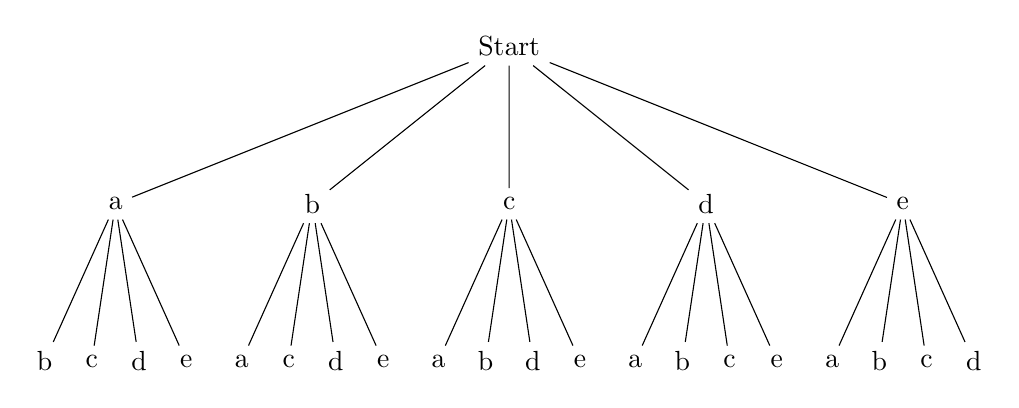
\begin{tikzpicture}[level distance=2cm,
  level 1/.style={sibling distance=2.5cm},
  level 2/.style={sibling distance=0.6cm}]
  \node {Start}
    child {node {a} child {node {b}} child {node {c}} child {node {d}} child {node {e}}}
    child {node {b} child {node {a}} child {node {c}} child {node {d}} child {node {e}}}
    child {node {c} child {node {a}} child {node {b}} child {node {d}} child {node {e}}}
    child {node {d} child {node {a}} child {node {b}} child {node {c}} child {node {e}}}
    child {node {e} child {node {a}} child {node {b}} child {node {c}} child {node {d}}};
\end{tikzpicture}


\easysubproblem{How many outcomes are in the above experiment? }

20 outcomes are in the above experiments. 

\intermediatesubproblem{Suppose we have five distinct elements, $a,b,c,d$ and $e$, and an experiment involves selecting two of these elements, one at a time, without replacement, and \textbf{disregarding} the order of selection. That is, selecting a $c$ and then selecting an  $e$ is the same as selecting an $e$ and then selecting a $c$. Does your diagram in part $(f)$ still apply? Explain your answer.}

No, the tree diagram from part f no longer applies to this version of experiment. The 

\intermediatesubproblem{Alice was asked the following question: From a group of three people, a president and two treasurers are to be chosen. How many outcomes are there? \\

Alice wrote down the following solution: 
\begin{tcolorbox}
We proceed in steps. 

\begin{enumerate}
    \item First choose a president. There are 3 choices.
    \item Then choose a treasurer. There are now 2 choices.
    \item Finally, choose a treasurer. There is now only 1 choice.
\end{enumerate}

By The Generalized Principle of Counting, there are $3 \times 2 \times 1 = 6$ choices.

\end{tcolorbox}

Draw a tree diagram and use the diagram to explain why Alice's solution is incorrect.}




\intermediatesubproblem{Prove that $P_{n,k} = \frac{n!}{(n-k)!}$.}


\end{enumerate}





\problem{In this exercise, we will answer a few counting problems.}


\begin{enumerate}

\easysubproblem{Each year starts on one of the seven days (Sunday through Saturday). Each year is either a leap year (i.e., it includes February 29) or not. How many different calendars are possible for a year?}


\easysubproblem{Three different classes contain 20, 18, and 25 students, respectively, and no student is a member of more than one class. If a team is to be composed of one student from each of these three classes, in how many different ways can the members of the team be chosen?}



\easysubproblem{ Five separate/distinct awards (best scholarship, best leadership qualities, and so on) are to be presented to selected students from a class of 30. How many different outcomes are possible if a student can receive any number of awards?}




\intermediatesubproblem{Suppose from $n$ distinct elements, an experiment consists of selecting $k$ of the elements, one at a time, \textbf{with} replacement. If the order of selection is noted, then how many different selections are possible? You may assume that $0 \leq k \leq n$ and $k \in \mathbb{Z}$.}



\easysubproblem{ Five separate/distinct awards (best scholarship, best leadership qualities, and so on) are to be presented to selected students from a class of 30. How many different outcomes are possible if each student can receive at most 1 award?}




\intermediatesubproblem{John, Jim, Jay, and Jack have formed a band consisting of 4 different instruments. If each of the boys can play all 4 instruments, then how many different arrangements are possible? }


\intermediatesubproblem{John, Jim, Jay, and Jack have formed a band consisting of 4 different instruments. John and Jim can play all 4 instruments, but Jay and Jack can only play the piano and drums. How many different arrangements are possible?}




\easysubproblem{Suppose you have 8 people labeled $A, B, C, D, E, F, G$ and $H$. In how many ways can 8 people be seated in a row if there are no restrictions on the seating arrangement?}


\hardsubproblem{Suppose you have 8 people labeled $A, B, C, D, E, F, G$ and $H$. In how many ways can 8 people be seated in a row if persons $A$ and $B$ must sit next to each other? Hint: Draw out 8 separate blocks where each block represents a person. Since $A$ and $B$ must sit together, consider them as one big block which is glued together. Now arrange these blocks. }








\extracreditsubproblem{Prove The Generalized Principle of Counting via induction.}

\end{enumerate}




\end{document}
